\section{Retrieval}
Besides of a collection of 0.7 billion bid phrases $P=\{p\}$ provided
by a commercial search engine, we extract a collection of 30 million
queries $Q=\{q\}$ from search logs. 
We offline expand $Q$ using $P$ (i.e., for each $q\in Q$, select
        several most related bid phrases from $P$).
Then we build index mapping each $q$ to its resulting expansions. 
When a query is issued by user, search engine look up the index,
     if the given query is in that index, its expansions (related bid
             phrases) are used to trigger ads for this query.
We also build up an online query expansion system, so when the
submitted query is unseen (not in $Q$), we retrieve related bid phrases for it
through our online system. 
%By conceptualization, we model both queries and bid phrases as concept
%vector and thus can measure similarity between short texts by
%measuring similarity between their corresponding concept vectors with
%conventional metrics.
%Like traditional IR system which builds inverted index mapping from
%words to documents, we can significantly improve the efficiency of
%retrieval by building inverted index mapping concepts to lists of bid
%phrases.
%However, in our setting, the number of bid phrases is on the order of
%a billion and some concepts contain extremely long inverted lists
%which incur significant overhead for building and accessing them.
%Moreover, according to our experiment, these popular concepts can't be
%treated as ``stop words'' and have to be reserved.
%Besides of offline expanding 30 million queries with 0.7 billion bid
%phrases for a commercial search engine, our aim is to construct a
%real-time query expansion system using billions of bid phrases.
%Thus the response time must be no more than tens of
%millisecond and the biggest challenge is efficiency.

No matter a query is processed offline or online, we divide the
retrieval procedure into two phases.
%We propose a two phase approach to find relevant bid
%pharases.%and our biggest challenge is scalability as the number of bid
%phrases is on the order of a billion and the online response time must
%be no more than hundreds of millisecond.  The two phases are as
%follows.
First, we find a small set of candidate bid phrases (somehow relevant) using some
semantic aware index.  Second, we rank candidates by measuring their
similarity with the given query and return the top-$K$ bid phrases.
%Candidates selection requires that our approaches should make
%compromise between effectiveness(mainly recall) and efficiency.
On the one hand, we want the set of candidates to be small enough so
that computational cost for ranking is minimized.  On the other hand,
the candidates should cover adequate relevant bid phrases.
%not miss optimal bid phrases and recall
%as many optimal ones as possible.
% Since the first phase reduces the number of bid phrases for further
% considered, conputational effort for ranking can satisfy the
% efficiency requirements of online system.
%function can compare pairs of short texts in a
%meticulous way while satisfing the efficiency requirement of onine
%system.
%In practice, any query expansion approach must be efficient enough to
%process billions of queries within a tolerable period.
%Regular solution for such efficiency requirement is building inverted
%index.
%In our setting, We should build lookup table through which we can find
%related bid keywords of a given concept efficiently.
%By conceptualization, we can derive a set of concepts for given query.
%Then we retrieve relevant bid keywords of those concepts using our
%preprocessed lookup table.
%Actually, the number of concepts of Probase is much smaller than the
%number of bid keywords to be processed and the numbers of related bid
%keywords of some general concepts\footnote{These concepts shouldn't be
%    treated as stop words like term-matching approach does} are so
%    large.
%As an extreme case, the most popular concept in Probase is associated
%with more than 200 millions of bid keywords when we apply our approach
%to 702 millions of bid keywords.
%Traditional "inverted index" solution can't satisfy efficiency
%requirement in our case duing to the serious overhead of scanning
%posting lists of popular concepts.
%
%
%
%For the above analysis, we use some sophisticated schemes to select a
%set of candidate bid keywords for each query firstly.
%The scale of candidates set should be small enough so that computing
%semantic-matching scores for candidates within it will not consume
%intolerable time.
%Then we rank these candidates according to their semantic-matching
%score with given query.
%In order to ensure the quality of candidates, we make full use of
%click log to select candidates for popular query.
%The relevance between candidates and given query is estimated by their
%co-click information derived by mining the click log.
%For queries(or bid keywords) which do not have enough click
%information to draw credible conclusion, we select candidates for them
%using locality-sensitive hash(LSH) scheme, which can be regarded as a
%compromise between effectiveness(mainly recall) and efficiency.
\subsection{Click Data based Retrieval}
\label{sec:CSCD}
We use click through data to help find relevant queries for a given
head query.  User clicks define strong associations between queries
and URLs~\cite{fuxman:keywordgeneration}.  Candidate selection using
click data (CSCD) is motivated by the assumption that queries leading
to clicks on the same URLs are semantically relevant.  We obtain
co-click data $\{(q,q',u,f)\}$ where $f$ is the number of times both
$q$ and $q'$ lead users to click $u$.
%We use the following rules to
%filter out some co-click data. 
%\begin{itemize}
%\item $f\geq$ a pre-set threshold. 
%\item $q$ and $q'$ share at least one common term
%\item Edit similarity between $q$ and $q'$ is larger than $0.1$.
%\end{itemize}
We then build inverted index for the co-click data.  Given a query at
runtime, we look it up in the index.  Assume the query exists in the
index. For each of its co-clicked queries, we check if it is a bid
phrase using {\it exact match}. If the query does not exist in the
index (it is a tail query), we turn to our second approach for {\it
  smart match}.
%As we know, the volume distribution of Web search queries follows the
%power law\cite{spink:theirqueries}.
%So there is no sufficient user behavior data(e.g., click data, session
%        data, etc.) for torso and tail queries.
%Worse, torso and tail queries constitute the majority and most of
%existing approaches do not do a good job on these ones.
%Indeed, We fail to select candidates for many queries due to their
%lack of sufficient click data.
\subsection{Concept Set based Retrieval}
\label{sec:CSJS}
%No matter a query is a head query or a tail query, we can
%conceptualize it into unit vector where each column corresponds to a
%concept in Probase.
%By conceptualization, we can transform a short text into a vector
%representation where each component correspond to a concept in
%Probase.
%By regarding the concept vector as a set where one concept belongs to
%it if the concept's corresponding coordinate is non-zero, 
By conceptualization, we transform each short text (either a query or
        bid phrase) into a set of concepts. 
Thus, we measure semantic similarity between two short
texts by measuring similarity between their corresponding concept
sets and do not distinguish a short text from its corresponding
concept set from now on.


%In our approach, 
We adopt Jaccard similarity
(JS$(p,q)=\frac{\vert{}p\cap{}q\vert{}}{\vert{}p\cup{}q\vert{}}$) and
set a threshold $t=0.8$ 
    %between their concept sets and do not distinguish a short text
    %from its corresponding concept set in the rest of this paper now.
%decide whether a query and a bid phrase is related.
%We set a threshold $t=0.8$ 
so that a bid phrases whose Jaccard
similarity with respect to the given query is no less
than $t$ qualifies for being the candidates of that query.
Thus, we can formalize our task as: 
\begin{definition}
Given a collection of bid phrases $P$, a collection of queries $Q$, a similarity
function ($\text{JS}(\cdot,\cdot)$), a threshold
$t=0.8$, to find all pairs of short texts $\{(p,q)\vert p\in P,q\in Q,
    \text{JS}(p,q)\geq t\}$ 
\end{definition}
A naive algorithm needs $O(\vert Q\vert\cdot\vert P\vert)$ comparisons (exactly computing Jaccard
    similarity) where $\vert P\vert$  is of billion order in our
setting. 
A popular solution is to convert Jaccard similarity constraint ($\text{JS}(p,q)\geq t$) into an equivalent
overlap constraint ($\text{O}(p,q)\geq\frac{t}{1+t}(\vert p\vert+\vert
            q\vert)=\alpha$) and build inverted index mapping each concept $c$
to a list of bid phrases that contain $c$. %in their corresponding concept sets. 
%a bid phrase qualifies for being candidate of a given query if the
%Jaccard Similarity between its concept set and the given query's
%concept set is no less than a threshold $t=0.8$.
%Thus, the task of selecting candidates for 30 million queries from
%0.7 billion bid phrases is a similarity join
%problem and we use PPJoin to find all pairs of short texts whose
%similarities are no smaller than $t$~\cite{xiao:ppjoin}.
% . is under the assumption that relevant search phrases are more
% likely to share similar concept sets.  We measure similarity between
% concept sets using Jaccard Similarity.  Jaccard Similarity between two
% concept sets $X$ and $Y$ is defined as follow:
%\begin{definition}
%\label{def:js}
%\begin{equation}
%\textnormal{Jaccard
%    Similarity}(X,Y)=\frac{\vert{}X\cap{}Y\vert{}}{\vert{}X\cup{}Y\vert{}}
%\end{equation}
%\end{definition}
%Obviously, we can't afford to apply Jaccard Similarity between the
%given query and every bid phrase.
%In such case, one solution is to build inverted index mapping concepts
%to bid phrases that contain them and apply efficient large scale
%similarity join algorithm such as PPJoin~\cite{xiao:ppjoin}.
%In detail, 
%and maintain a inverted index
%mapping a concept $c$ to a list of short texts that contain $c$.  
We scan each query $q\in Q$,
   probing the index using every concept of $q$, and obtain
   a set of bid phrases; merging these bid phrases together gives us
   their actual overlap with $q$, final results
   can be extracted by removing bid phrases whose overlap with $q$ is
   less than $t$.
However, some concepts contain extremely long inverted lists
which incur significant overhead for building and accessing them.
Moreover, according to our experiment, these popular concepts can't be
treated as ``stop words'' and thus have to be reserved. 
For large scale efficient similarity join, we adopt 
%By the filtering rules of PPJoin, the number of bid phrases that
%need verification (actually computing Jaccard Similarity) is
%significantly reduced.
PPJoin~\cite{xiao:ppjoin} which proposed several filtering rules 
allowing us to scan only part of a concept's inverted list, to prune a
considerable number of bid phrases in the inverted lists before
actually computing Jaccard similarity.  Thus, the computaional
effort for exactly comparison is significantly reduced.

%Although we use this technique to expanded 30 million queries with
%0.7 billion bid phrases within an acceptable period of time, these exact similarity
%search approaches seem not efficient enough.
%In order to make large scale similarity search efficiently,

Constructing online query expansion system means for a query, we must
select its most related bid phrases from $P$ within tens of
millisecond.  Besides of the scalability of $P$, the not small number
of elements of a concept set is also a challenge.  For a given query
$q$, to efficiently select candidates $\{p\vert p\in
P,\text{JS}(p,q)\geq t\}$, we give up those exact algorithms that have
to merge hundreds of posting lists of inverted index and adopt
locality-sensitive hash (LSH) which is \emph{approximate} algorithm
for finding similar items.
    %under some distance.
%  However, optimal solution is not as attractive as quickly
% retrieving a set of candidates with high enough quality.  We can
% ensure the precise and recall to some extend from probability
% perspective by setting several parameters of LSH tables appropriately.

% Although there are a lot of materials~\cite{raja:massivedatasets} presenting details of LSH, we
% give a brief introduction here for readers' convenience.
%We represent concept sets by a 0-1 matrix where each column represents
%one concept set and each row corresponds to one concept of Probase.
%There is a $1$ in row $r$ and column $c$ when the concept of $r$ is
%one element of concept set of $c$.
We represent a concept set by a 0-1 vector where each component
corresponds to one concept of Probase. 
There is a $1$ in row $r$ when the corresponding concept of row $r$ is
one element of the concept set.
When we apply a minhash function $f(\cdot)$ to the 0-1 vector of a
concept set, it applies a permuation over the rows of it.
The minhash value of any vector (concept set) is the subscript of the
first row in the permuted order in which the value is $1$.
The most important property of minhash function $f(\cdot)$ is that
\begin{equation}
\label{eqn:minhashjs}
\Pr[f(p)=f(q)]=\text{JS}(p,q)
\end{equation}
%\vspace{-15pt}
%\begin{proof}
%Classify the rows of matrix representation into three classes:
%$\alpha$: both $X$ and $Y$ contain the concept of this row; $\beta$:
%only one of $X$ and $Y$ contains the concept of this row; $\gamma$:
%the concept of this row isn't included by neither $X$ nor $Y$.
%
%Obviously, according to definition \ref{def:js} we have:
%\begin{equation}
%\label{eqn:js1}
%\textnormal{Jaccard Similarity}(X,Y)=\frac{\vert\alpha\vert}{\vert\beta\vert+\vert\alpha\vert}
%\end{equation}
%
%On the other hand, based on the definition of minhash function,
%   $Pr[f(X)=f(Y)]=$ the fraction of ramdon permutations that rank the first
%   row of class $\alpha$ ahead the first row of class $\beta$.
%Thus, we have:
%\begin{equation}
%\label{eqn:minhash}
%\Pr[f(X)=f(Y)]=\frac{\vert\alpha\vert}{\vert\beta\vert+\vert\alpha\vert}
%\end{equation}
%
%The Eq.\eqref{eqn:js1} and Eq.\eqref{eqn:minhash} ensure the validation
%of Eq.\eqref{eqn:minhashjs}
%\end{proof}
%As \cite{raja:massivedatasets} defined:
%\begin{definition}
%A family $\mathcal{F}$ of functions is $(d_1,d_2,p_1,p_2)-sensitive$
%if $\forall f\in\mathcal{F}$:\\
%$d(x,y)\leq d_1\rightarrow Pr[f(x)=f(y)]\geq p_1$\\
%$d(x,y)\geq d_2\rightarrow Pr[f(x)=f(y)]\leq p_2$
%\end{definition}
Minhash function family $\mathcal{F}$ consists of minhash functions
$f(\cdot)$ each manipulates concept sets with different permutation.
%Since Jaccard Distance is defined as one minus Jaccard Similarity, we
%can use Jaccard Similarity's minhash function family as
%$(d_1,d_2,1-d_1,1-d_2)-sensitive$ LSH family for Jaccard Distance.
%When $d_1<d_2$ which implies $p_1=1-d_1>p_2=1-d_2$, it will be useful
%for similar sets are more likely to be mapped into the same buckets.



To ensure acceptable precision and recall, we use the banding
technique~\cite{raja:massivedatasets} to ``amplify'' the LSH family. By
randomly choosing $n(n=r\ast b)$ minhash functions
$f_{i,j}\in\mathcal{F},i=1,\ldots,r\textnormal{ and }j=1,\ldots,b$ and
dividing them into $b$ bands each of $r$ functions, we define the
collision (i.e., with same LSH signature) of two concept sets:
%LSH signature as follow:
%\begin{definition}
%$Sig(\cdot)=(B_{1}(\cdot),\ldots,B_{b}(\cdot))$ where $B_{i}(\cdot)=(f_{i,1}(\cdot),\ldots,f_{i,r}(\cdot))$
%\end{definition}
%We also define the collision(with the same signature) of two sets:
\begin{definition}
\label{def:col}
%$Sig(q)=Sig(w)\Leftrightarrow{}\exists i\in
%1,\ldots,b, B_{i}(q)=B_{i}(w) \textnormal{ where }\forall i,
%    B_{i}(q)=B_{i}(w)\Leftrightarrow\forall j\in1,\ldots,r,
%    f_{i,j}(q)=f_{i,j}(w)$
$\text{Sig}(p)=\text{Sig}(q)\Leftrightarrow{}\exists i\in 1,\ldots,b$ s.t. $\forall
j\in 1,\ldots,r,f_{i,j}(p)=f_{i,j}(q)$
\end{definition}
Suppose the $\text{JS}(p,q)=d$, according to Definition \ref{def:col}, the probability of their
collision is $1-(1-d^r)^b$ which is a sharp S-curve (see Figure
        \ref{fig:scurve} for example where $r=8, b=16$).  
%Since we believe that
%bid phrases whose corresponding concept sets achieve no less than 
%$0.8$ Jaccard Similarity with respect to given query's concept set are
%suitable to be candidates, 
We should set $r$, $b$ appropriate values such that %the collision probabilities of true
%candidates (JS$(b,q)\geq t$) near $1$.
$\Pr[\text{Sig}(p)=\text{Sig}(q)]$ near $1$ for $(p,q)$ that satisfies
$\text{JS}(p,q)\geq t$ while those not so similar bid phrases have low
collision probabilities because recalled many false candidates will increase the
computational effort (exactly computing the similarity) which means
depression of efficiency.
%Considering that those with less than $0.5$ Jaccard Similarity are so
%irrelevant,
%Based on above consideration, we choose parameters $r=8$, $b=16$ for
%our LSH tables.
\begin{figure}
\centering
%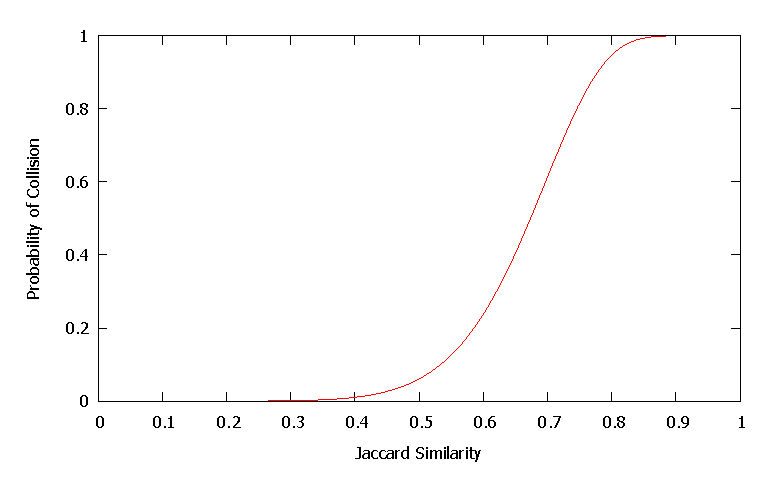
\epsfig{file=figures/scurve.eps, width=1.5in, height=1.3in}
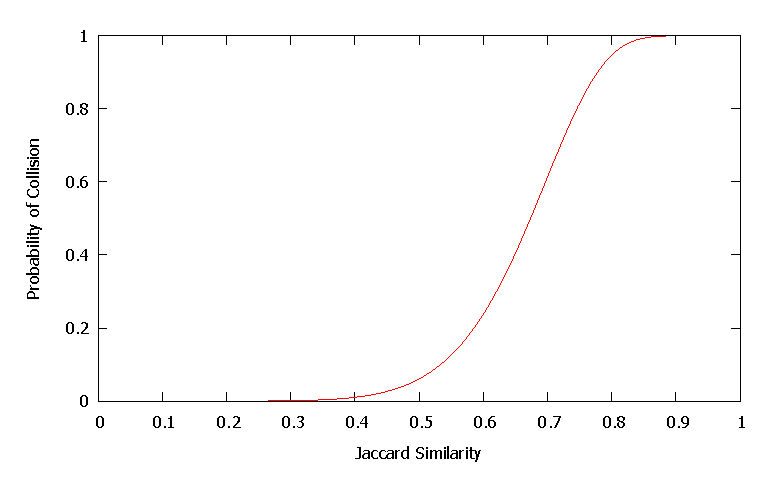
\includegraphics[width=1.5in, height=1.3in]{figures/scurve.eps}
\caption{$\Pr[\textnormal{Sig}(p)=\textnormal{Sig}(q)]=1-(1-d^r)^b$}
\label{fig:scurve}
\end{figure}
%The curve that Jaccard Similarity of two concept sets versus
%probability that their LSH signatures collide is illustrated in Figure
%\ref{fig:scurve}.



%We pre-compute LSH signatures for bid phrases' corresponding
%concept sets and build the LSH tables.
We pre-compute LSH signatures for $p\in P$.%bid phrases' corresponding concept
%sets.
For each band, we firstly aggregate bid phrases that have identical signature.
Then we maintain the index by a key-value pair memory object caching
system where signatures are used as keys and lists of
aggregated bid phrases are used as values.
We maintain the index of each band in one specific machine.
%inverted index by which, given the LSH signature
%of the given query's concept set, we can efficie-ntly retrieve bid
%phrases whose corresponding concept sets are mapped into the same
%buckets.
At runtime, when a query is posed, we compute its concept set's LSH
signature and distribute signature of each band to corresponding machine.
%and use the signature to retrieve bid phrases through our hash tables.
For each band, we check whether the signature of query happens to be
the key of a certain key-value pair.
If it is the case, value (i.e., list of bid phrases) of the pair is
returned because these bid phrases have large Jaccard similarity with
the query under some probabilistic guarantee.
Finally, we select at most hundreds of bid phrases from results
returned from different bands and compute exact Jaccard Similarity for
them to select true candidates.
%True positive ones are selected as candidates.
%The disjunctive relationship between different bands enables us to
%process each of them seperately.
By the LSH scheme, we replace cumbersome calculation such as merging
hundreds of posting lists of inverted index by %several access to only
%a few hash tables.
accessing $b$ hash tables.
Besides, the scalability of our approach partly relies on the banding
technique because the disjunctive relationship between different bands enables
us to maintain each band in one machine and process in a parallel way.
It is this feature that improves the scalability and efficiency of our
system.
%Since these selected candidates are unordered.
%We rank them by computing their exact Jaccard Similarity with respect
%to query's concept set and rank them in descending order and only reserve
%at most about one hundred of them.
%The connection between short text and concepts can be modeled as a
%bipartite graph and organized in adjacent lists which can be stored in
%distributed key-value pair in-memory storage system(e.g., memcached)
%    easily when the scale of corpus is too large to be held in memory
%    of one machine.
\subsection{Ranking}
%In fact, we can simply rank candidates by Jaccard similarity between
%their concept sets and the given query's.  Since Probase is a
%probabilistic taxonomy, measuring similarity between concept sets only
%exploits its rich isA relationships but hasn't made full use of its
%typicalities.
We assign a semantic-matching score (SMS) to each candidate bid phrase
with respect to a given query.  Then we rank these candidates by their
assigned SMS score in descending order and select top ranking bid
phrases.  Intuitively, SMS should be proportional to the semantic
similarity between short texts.  Since each short text is
characterized by a concept vector, we can estimate the similarity
between short texts by measuring the similarity between their
corresponding concept vectors.  Formally, for a given query $q$ and a
bid phrase $p$, with their corresponding concept vectors denoted as
$\mathbf{c_q}$ and $\mathbf{c_p}$, SMS is defined as follows:
\begin{definition}
\begin{equation}
\textnormal{SMS}(q,p)=\cos(\mathbf{c_q},\mathbf{c_p})=\mathbf{c_q}\cdot\mathbf{c_p}
\end{equation}
\end{definition}
%By filtering a large portion of bid keywords and only reserving a
%handful of high-quality candidatas which seem to be relevant to given
%query, we can compute SMS for candidates with respect to given query
%in a meticulous way while satisfing the efficiency requirement of
%online system.\\
%
%
%
%Firstly, we distinguish head instances from tail instances to
%re-weight concepts derived from these observed instances.
%In contrast of classic term weighting scheme such as TF-IDF which
%measures significance of a word to a certain document based on the
%frequence of the word within the content of the document as well as
%the frequency of the word in the whole corpus, we determine the
%significance of each instance according to its functionality with
%respect to expressing the meaning of the short text.
%For example, short text ``angry birds for windows phone 7'' refers to
%the ``wp7'' version of a popular game named ``angry birds''. Here
%``angry birds'' is a head instance but ``windows phone 7'' is a modifier
%instance.
%By semantically re-weight associated concepts of each short text, we
%can target the core meaning of short text more accurately.
%We present our work on distinguishing head/modifier in another
%paper.
%
%
%
%Since taxonomy used in our approach organizes concepts hierarchically
%by ``is-A'' relation, regarding each concept as a independent
%coordinate and adopting conventional metrics(e.g., cosine) to measure
%similarity between two concept vectors seems unreasonable.
%Search users with identical search intent but different extent of
%expertise may issue different queries.
%For example, customer has no idea about ``kindle'' may issue query
%``amazon ebook reader'' and ``kindle'' is more specific but still so
%relevant to his/her query.
%In order to exploit more specific or more general bid phrases to
%answer given query, we measure similarity between short texts with
%consideration of not only their corresponding concept vector but also both their parent concepts and children concepts.
%Given a concept vector $\mathbf{c}$, we denote its corresponding
%concept set as
%$C_{\mathbf{x}}=\{(c_1,w_1),(c_2,w_2),\ldots,(c_n,w_n)\}$ where
%$\forall i\in 1,\ldots,n,w_i>0$.
%We derive parents of $C_{\mathbf{x}}$ by regarding concepts within it
%as entities and ranking their hypernyms by equation
%\ref{eqn:naivebayesian}.
%Children of $C_{\mathbf{x}}$ is derived by ranking hyponyms of its
%concepts by:
%\begin{equation}
%P(e\vert C_{\mathbf{x}})=\frac{P(e)P(C_{\mathbf{x}}\vert
%        e)}{P(C_{\mathbf{x}})}\propto P(e)\prod_{i}^{n}P(c_i\vert e)
%\end{equation}
%Then we transform parents and children of $C_{\mathbf{x}}$ into
%concept vector form and normalize them resulting
%$\mathbf{x}_{\textnormal{p}},\mathbf{x},\mathbf{x}_{\textnormal{c}}$.
%Given two concept vectors $\mathbf{x}$ and $\mathbf{y}$, we define the
%SMS of them as:
%\begin{definition}
%SMS($\mathbf{x},\mathbf{y}$)=$\max_{t\in\{\mathbf{x}_{\textnormal{p}},\mathbf{x},\mathbf{x}_{\textnormal{c}}\}\times\{\mathbf{y}_{\textnormal{p}},\mathbf{y},\mathbf{y}_{\textnormal{c}}\}}\cos(t)$
%\end{definition}


%%% Local Variables:
%%% mode: latex
%%% TeX-master: "adselection"
%%% End:
